\chapter{الفوتونات والفونونات}\label{ch:b3:photons-phonons}

وُلدت النظرية الكمومية في موضوع هذا الفصل. ففي سنة 1900 أبى
طيف الأجسام المتوهجة أن يطيع الفيزياء الكلاسيكية ---
بل أسوأ، إذ تنبأت الفيزياء الكلاسيكية بطاقة \emph{لانهائية} عند
الأطوال الموجية القصيرة، وهي ``كارثة فوق البنفسجي'' --- وتبيّن أن دواء بلانك
اليائس، أي طاقة في رزم مقدارها $h\nu$، هو
مفتاح القرن الرئيسي. ومع الآلة المجمَّعة الآن --- من إحصاء
الأنماط في \cref{ch:b3:schrodinger-three-dimensions}، وترموديناميك
المذبذب في \cref{ch:b3:canonical-ensemble} --- يأخذ \omterm{thm:b3:photons-phonons:planck}{قانون بلانك}
نصف صفحة: أي غاز من الفوتونات، بمذبذب واحد مشغول بوزونيًّا
لكل نمط من أنماط الجوف. ونصف الصفحة نفسه، مع الصوت مكان الضوء،
هو نظرية ديباي في الأجسام الصلبة والسعة الحرارية $T^3$ التي أخطأها
نموذج أينشتاين. ويملأ كلَّ سنتيمتر مكعب من الكون
تحفةُ الموضوع: خلفية الكون الميكروية عند 2.725 كلفن،
وهي أكمل جسم أسود قيس قط --- أي
الإشعاع الحراري للكون الفتيّ نفسه، ولا يزال يصل.

\section{قانون بلانك، مستنتَجًا}

\begin{theorem}[طيف الجسم الأسود]\label{thm:b3:photons-phonons:planck}
\index{قانون بلانك}\index{إشعاع الجسم الأسود}
الجوف عند درجة الحرارة $T$ يسند أنماطًا كهرمغناطيسية ---
أي أمواجًا موقوفة تُحصى تمامًا كما في
\cref{prop:b3:schrodinger-three-dimensions:counting}، مرتين من أجل
الاستقطاب:
\[
g(\nu)\,\dd\nu = \frac{8\pi V}{c^3}\,\nu^2\,\dd\nu .
\]
وكل نمط مذبذب كمومي يحمل، عند التوازن،
$\bar n = 1/(\eu^{h\nu/k_{\text{B}}T} - 1)$ فوتونًا
(\cref{exo:b3:canonical-ensemble:5}؛ أو بالمكافئ، بوزونات عند $\mu =
0$). فتكون الطاقة لكل حجم ولكل تواتر
\[
u(\nu, T) = \frac{8\pi h\nu^3}{c^3}\,
\frac{1}{\eu^{h\nu/k_{\text{B}}T} - 1} :
\]
وهو \emph{\omterm{thm:b3:photons-phonons:planck}{قانون بلانك}} (1900). ونتائجه، وكلها كما قيست:
الذروة عند $\lambda_{\max}T = \qty{2898}{\micro m.K}$ (وهو قانون
فين للانزياح في كتاب السنة الثانية، مستنتَجًا الآن)؛ والتدفق الكلي
من سطح أسود $\Phi = \sigma T^4$ مع
\[
\sigma = \frac{2\pi^5k_{\text{B}}^4}{15h^3c^2}
 = \qty{5.67e-8}{W.m^{-2}.K^{-4}}
\]
(ستيفان--بولتزمان، وثابته مبنيّ الآن من $h$ و $c$ و
$k_{\text{B}}$)؛ وكثافة الفوتونات $n_\gamma \approx
\num{2.03e7}\,(T/\unit{K})^3$ في المتر المكعب.
\end{theorem}

\begin{proof}[برهان جزئي]
اضرب إحصاء الأنماط في $h\nu\,\bar n$. ويعطي تكامل
الطاقة الكلي، مع $x = h\nu/k_{\text{B}}T$ و $\int_0^\infty
x^3\dd x/(\eu^x - 1) = \pi^4/15$ (مقبولًا)، المقدارَ $u_{\text{كلي}}
= aT^4$ ويعطي، مع عامل التدفق المعياري $c/4$، الثابتَ
$\sigma$ المذكور. وأما قانون فين فهو تعظيم
\cref{exo:b3:photons-phonons:1}. وعند التواتر المنخفض ($h\nu \ll
k_{\text{B}}T$) يحمل كل نمط $k_{\text{B}}T$ ---
أي رايلي--جينز، وهو صحيح للراديو، وكارثي إذا مُدّ إلى كل
$\nu$: فقطع بلانك هو سحب رخصة التوزّع المتساوي
(\cref{thm:b3:canonical-ensemble:equipartition})
نمطًا نمطًا.
\end{proof}

\begin{omfigure}
\begin{tikzpicture}
  \begin{axis}[omaxis, axis x line=bottom, axis y line=left,
    width=11.4cm, height=6.0cm, xmin=0, xmax=4.4, ymin=0, ymax=1.5,
    xlabel={$\nu$ (بوحدات $10^{14}$ Hz)}, ylabel={$u(\nu)$ (محجَّمًا)},
    xlabel style={at={(axis description cs:0.5,-0.09)}, anchor=north},
    xtick={1,2,3,4}, ytick=\empty, clip=false,
    legend style={font=\scriptsize, at={(0.97,0.93)}, anchor=north east,
      draw=none, fill=none}]
    \addplot[omDef, very thick, domain=0.01:4.4, samples=200]
      {1.42*x^3/(exp(x/1.208)-1)/8.3};
    \addlegendentry{$T = \qty{5800}{K}$ (الشمس)}
    \addplot[omThm, thick, domain=0.01:4.4, samples=200]
      {1.42*x^3/(exp(x/0.833)-1)/2.72};
    \addlegendentry{$T = \qty{4000}{K}$}
    \addplot[omExo, thick, domain=0.01:4.4, samples=200]
      {1.42*x^3/(exp(x/0.625)-1)/1.15};
    \addlegendentry{$T = \qty{3000}{K}$}
    \addplot[gray, dashed, domain=0.01:1.9, samples=100]
      {1.42*x^2*1.208/8.3};
    \node[gray, font=\scriptsize, anchor=west, rotate=48] at (axis cs:1.28,0.62)
      {رايلي--جينز};
  \end{axis}
\end{tikzpicture}

{\small أطياف بلانك عند ثلاث درجات حرارة (كلٌّ محجَّم إلى
ارتفاع مقارن: فالمساحات الحقيقية تنمو وفق $T^4$). ويتبع خط
رايلي--جينز الكلاسيكي الجناح المنخفض التواتر ثم
يحلّق نحو كارثة فوق البنفسجي؛ أما رسم بلانك $h\nu$ فيغلق
الأنماط العالية التواتر ويثني المنحني نزولًا.}
\end{omfigure}

\begin{example}[ثلاثة موازين حرارة]\label{ex:b3:photons-phonons:thermometers}
الشمس ($T = \qty{5800}{K}$): ذروتها عند \qty{0.50}{\micro m} ---
وقد تطورت أعيننا على أعظميتها. وجسم عند \qty{310}{K}: ذروته
قرب \qty{9.4}{\micro m}، ويشعّ $\sigma T^4 \approx
\qty{520}{W/m^2}$ من كل متر مربع من الجلد (ورحمةً بنا،
تشعّ الغرفة راجعةً؛
\cref{exo:b3:photons-phonons:2}). والكون ($T =
\qty{2.725}{K}$): ذروته قرب \qty{1.9}{mm} بالصورة التواترية
(\qty{160}{GHz})، و $411$ فوتونًا في السنتيمتر المكعب ---
أي خلفية الكون الميكروية، وهي المثال الكبير في هذا الفصل
(\cref{pb:b3:photons-phonons:1}).
\end{example}

\begin{proposition}[ترموديناميك الضوء]\label{prop:b3:photons-phonons:thermo}
\index{ضغط الإشعاع!الحراري}
لغاز الفوتونات كثافة طاقة $u = aT^4$ (مع $a =
4\sigma/c$)، وضغط
\[
P = \frac u3 ,
\]
وكثافة إنتروبيا $\tfrac43 aT^3$، وعدد فوتونات $\propto T^3$.
والنتائج: أن علبة مملوءة إشعاعًا تتمدد تمددًا كظومًا
تبرد وفق $T \propto 1/L$ --- فقد بردت فوتونات الكون المتمدد
من $3000$ كلفن إلى $2.725$ كلفن اليوم بعامل مطّ
$\approx1100$ مع \emph{إبقائها} على طيف بلانك تامّ؛ و
في النجوم الضخمة يتيح النموّ $T^4$ لضغط الإشعاع أن ينافس
ضغط الغاز، فيضع حدًّا أعلى لكتل النجوم
(\cref{ch:b3:astrophysics}).
\end{proposition}

\begin{proof}[برهان جزئي]
$P = u/3$: فالغاز المتماثل المناحي من جسيمات بسرعة $c$ يعطي
ثلث كثافة طاقته ضغطًا (وهو العامل $\langle
\cos^2\theta\rangle = 1/3$، كما في النظرية الحركية في كتاب
السنة الأولى). والإنتروبيا من $\dd U = T\dd S - P\dd V$ مطبَّقة على $U =
aT^4V$. وأما الكظوم: فثبات $S \propto T^3V$ يعطي $T \propto
V^{-1/3}$.
\end{proof}

\section{الفونونات: إتمام ديباي}

\begin{theorem}[نموذج ديباي]\label{thm:b3:photons-phonons:debye}
\index{نموذج ديباي}\index{فونون}
اهتزازات البلورة \omterm{prop:b3:continuum-elasticity:waves}{أمواج مرنة} مكمَّمة تمامًا مثل
الضوء: أي \emph{فونونات}، بثلاثة استقطابات عند سرعة الصوت
$c_{\text{s}}$، تُحصى مثل الفوتونات لكن بسقف كلي مقداره
$3N$ نمط --- وهو السقف الذي يعرّف \emph{درجة حرارة ديباي}
\[
k_{\text{B}}\theta_{\text{D}} = \hbar c_{\text{s}}
(6\pi^2n)^{1/3} .
\]
وتُقحم السعة الحرارية بين القانونين الكلاسيكيين:
\[
C \to 3Nk_{\text{B}} \;(T \gg \theta_{\text{D}})
\qquad\text{(ديولونغ--بتي)} ,
\qquad
C \to \frac{12\pi^4}{5}\,Nk_{\text{B}}
\Big(\frac{T}{\theta_{\text{D}}}\Big)^3
\;(T \ll \theta_{\text{D}}) :
\]
أي قانون $T^3$ الذي طالبت به مسعّرية درجات الحرارة المنخفضة و
عجز عنه تواتر أينشتاين الواحد
(\cref{exo:b3:canonical-ensemble:6}). والسبب هو نفسه
سبب الضوء: فمهما بردت البلورة، توجد كمّات صوت
طويلة الموجة رخيصة كيفما شئنا، ويعطي إحصاؤها الشبيه بالفوتونات
قانونَ $T^3$ الشبيه بالفوتونات.
\end{theorem}

\begin{proof}[برهان جزئي]
كرّر حساب الفوتونات مع $c \to c_{\text{s}}$، وثلاثة
استقطابات، ومجموع أنماط $\int g\,\dd\nu = 3N$ يثبّت
القطع. وعند $T \ll \theta_{\text{D}}$ يكون القطع غير مرئي و
يعطي تكامل الطاقة $T^4$ المقدارَ $C \propto T^3$؛ وعند $T$ المرتفعة يحمل كل
نمط من الأنماط $3N$ المقدارَ $k_{\text{B}}T$. وأما تكامل
الإقحام الكامل فمقبول.
\end{proof}

\begin{omfigure}
\begin{tikzpicture}
  \begin{axis}[omaxis, axis x line=bottom, axis y line=left,
    width=11.0cm, height=5.6cm, xmin=0, xmax=1.5, ymin=0, ymax=1.15,
    xlabel={$T/\theta_{\text{D}}$}, ylabel={$C/3Nk_{\text{B}}$},
    xlabel style={at={(axis description cs:0.5,-0.1)}, anchor=north},
    xtick={0.5,1,1.5}, ytick={0.5,1}, clip=false,
    legend style={font=\scriptsize, at={(0.95,0.42)}, anchor=north east,
      draw=none, fill=none}]
    \addplot[gray, dashed, domain=0:1.5, forget plot] {1};
    \addplot[omDef, very thick, domain=0.02:1.5, samples=200]
      {1/(1+0.01283/(x*x*x))};
    \addlegendentry{ديباي}
    \addplot[omExo, thick, dashed, domain=0.02:1.5, samples=200]
      {(0.75/x)^2*exp(-0.75/x)/(1-exp(-0.75/x))^2};
    \addlegendentry{أينشتاين}
    \node[omDef, font=\scriptsize, anchor=west] at (axis cs:0.2,0.28)
      {$\propto T^3$};
    \draw[->, omDef] (axis cs:0.2,0.24) -- (axis cs:0.13,0.13);
  \end{axis}
\end{tikzpicture}

{\small السعة الحرارية لبلورة: يبلغ النموذجان كلاهما
ديولونغ--بتي، لكن عند درجة الحرارة المنخفضة يموت منحني أينشتاين
ذو التواتر الواحد موتًا أُسّيًا بينما تسند فونونات ديباي
الرخيصة الطويلة الموجة قانونَ $T^3$ المقيس --- فمنطقة $T$ المنخفضة
``فيزياء فوتونات'' محضة بالصوت.}
\end{omfigure}

\begin{example}[الفونونات جسيمات حقيقية]\label{ex:b3:photons-phonons:phonon-real}
تنتثر الفونونات النيوترونات والأشعة السينية مع حفظ الطاقة و(كمية
الحركة) البلورية --- ومنحنيات التبدد المقيسة
$\omega(\vect k)$ في \cref{ch:b3:crystalline-solids} هي
تحليلها الطيفي. وهي تحمل الحرارة: فناقلية العازل الحرارية
هي ناقلية غاز فونونات $\kappa = \tfrac13 Cc_{\text{s}}\ell$، و
الألماس --- الصلب الخفيف النقيّ --- ينقل خمسة أضعاف النحاس عند
حرارة الغرفة بالفونونات وحدها
(\cref{exo:b3:photons-phonons:12}). وهي تخبو عند درجة الحرارة
المنخفضة وفق $T^3$، ولذلك يتحدث مهندسو التبريد عن
بلورات تصير ``صامتة صوتيًّا''.
\end{example}

\begin{method}[حرفة غاز الإشعاع]\label{met:b3:photons-phonons:method}
(1) أحصِ الأنماط ($\propto\nu^2$ لكل استقطاب في ثلاثة أبعاد)؛ واشغلها
بالمقدار $1/(\eu^{\beta h\nu} - 1)$؛ وكامل --- وتوقّع طاقات $T^4$
وأعدادًا وسعات $T^3$. (2) والذُّرى بفين؛ و
المجاميع بستيفان؛ ولا يكون $k_{\text{B}}T$ الكلاسيكي لكل نمط إلا تحت
$h\nu \sim k_{\text{B}}T$. (3) ومن أجل الأجسام الصلبة، اسقف الأنماط عند $3N$
(أي عند $\theta_{\text{D}}$)؛ وصورة أينشتاين من أجل أنماط الفرع الضوئي،
وصورة ديباي من أجل الصوتي. (4) والإشعاع الكظوم: $T \propto
V^{-1/3}$. (5) وتحقق من ثابتَي الصنعة: $\lambda_{
\max}T = \qty{2898}{\micro m.K}$ و $\sigma =
\qty{5.67e-8}{W/m^2K^4}$.
\end{method}

\begin{omfigure}
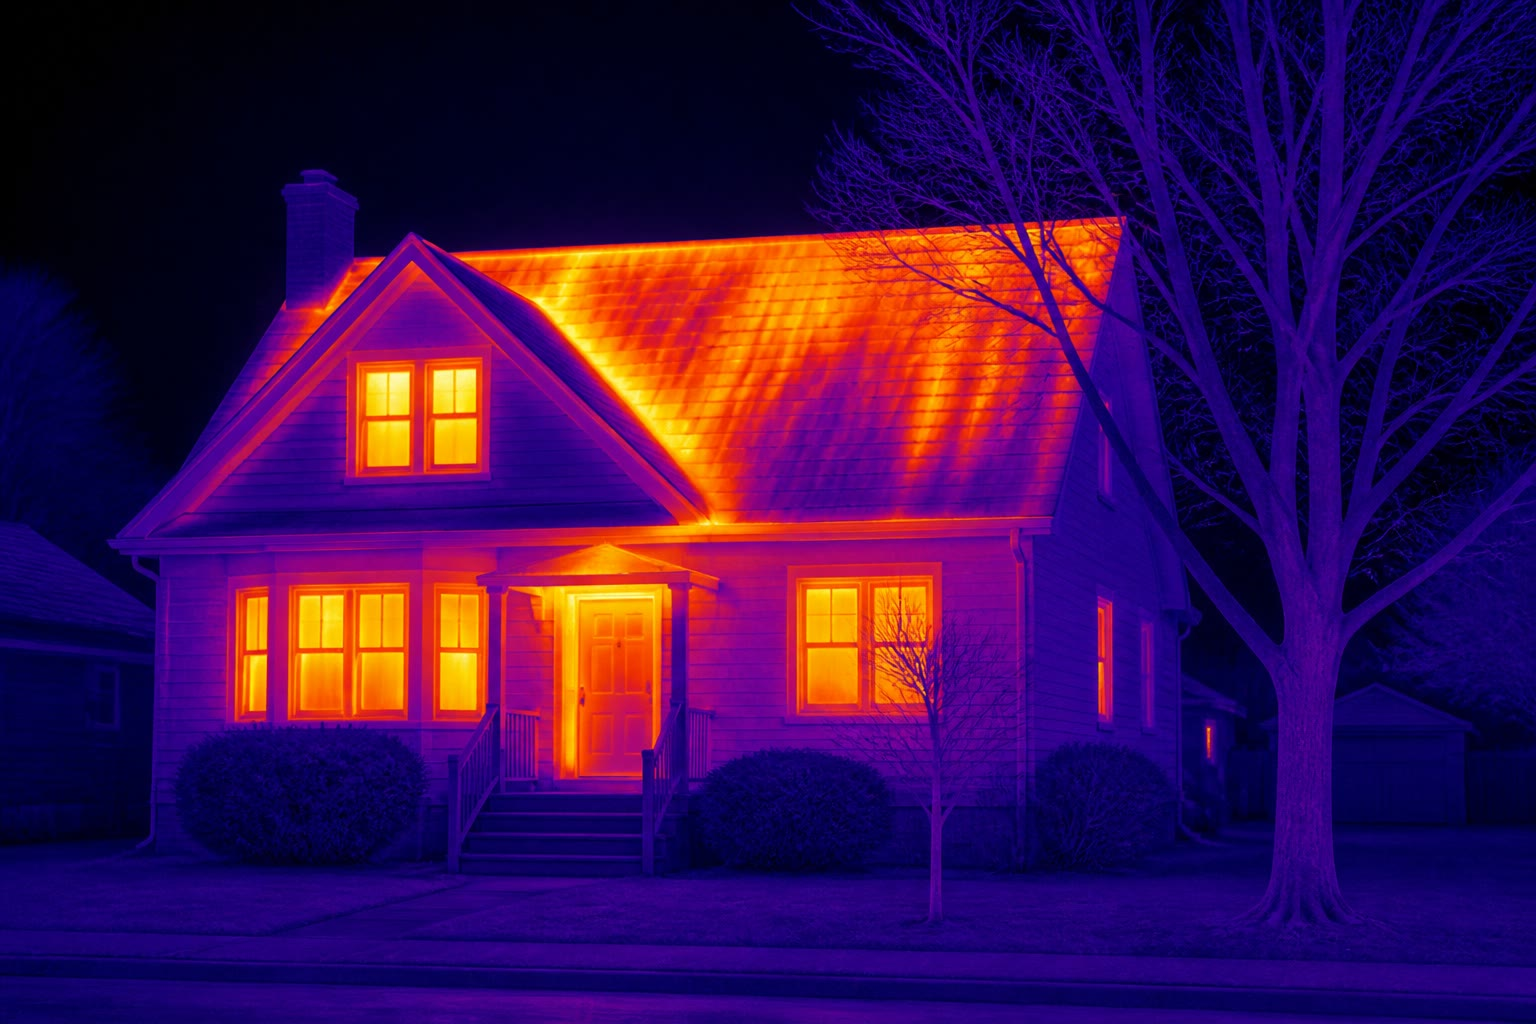
\includegraphics[width=0.58\linewidth]{images/book5/ai/b5-09-thermal-house.jpg}

{\small بيت من خلال آلة تصوير حرارية: كل سطح يشعّ طيف بلانك الخاص به، وتقرأ الآلة درجة الحرارة من الأشعة تحت الحمراء مباشرةً --- أي ستيفان وبولتزمان وفين يدقّقون فاتورة التدفئة.}
\end{omfigure}

\section{تمارين}

\begin{exercise}[$\star$]\label{exo:b3:photons-phonons:1}
(أ) من \omterm{thm:b3:photons-phonons:planck}{قانون بلانك} بصورة الطول الموجي، بيّن أن الذروة تطيع
$\lambda_{\max}T = $ ثابت (ويمكن الاستشهاد بالمعادلة المتساميّة:
$x = 4.965$). (ب) احسب الأطوال الموجية الذروية من أجل
الشمس، وفتيلة عند \qty{2700}{K}، وجسم عند \qty{310}{K}، وسماء
عند \qty{2.725}{K}. (ج) وأيّ الأربعة تعاينه العين البشرية
جيدًا، وما نسبة خرج الفتيلة المرئية
(قدّرها: صغيرة)؟ (د) ولماذا تكون ``آلات التصوير تحت الحمراء'' الأداة
المناسبة للناس والمباني؟
\end{exercise}

\begin{exercise}[$\star$]\label{exo:b3:photons-phonons:2}
الميزانيات الإشعاعية. (أ) شخص ($\qty{1.7}{m^2}$، وجلده عند
\qty{306}{K}) في غرفة عند \qty{293}{K}: احسب القدرة المشعّة الصافية
$\sigma A(T_1^4 - T_2^4)$. (ب) قارنها بأيض الجسم البالغ
\qty{100}{W}: فلماذا نحتملها (بالملابس، و
بالغرفة التي تشعّ راجعةً)؟ (ج) تمتصّ الأرض ضوء الشمس على $\pi
R^2$ وتشعّ على $4\pi R^2$: استنتج $T_{\text{فعّال}}
= [(1-A)\,\Phi_\odot/4\sigma]^{1/4}$ مع $\Phi_\odot =
\qty{1361}{W/m^2}$ وبياض $A = 0.30$، ثم احسبها. (د) والمتوسط
السطحي المقيس \qty{288}{K}: سمِّ آلية
الفرق البالغ \qty{33}{K}
(\cref{pb:b3:harmonic-oscillator:1}).
\end{exercise}

\begin{exercise}[$\star$]\label{exo:b3:photons-phonons:3}
عدّ الفوتونات. (أ) مع $n_\gamma = \num{2.03e7}\,T^3$ في
المتر المكعب: احسب كثافة فوتونات الخلفية عند \qty{2.725}{K}.
(ب) وضوء الشمس عند الأرض: من $\Phi_\odot$ ومن متوسط طاقة فوتون
$\approx 2.7\,k_{\text{B}}T_\odot \approx \qty{1.35}{eV}$،
احسب تدفق الفوتونات لكل متر مربع في الثانية. (ج) ومصباح
متوهج عند \qty{60}{W} (ونسبة المرئي منه 5\%): احسب الفوتونات المرئية في
الثانية. (د) ولماذا يكون ``عدّ الفوتونات'' روتينيًّا لعلماء الفلك
وسخيفًا للمدافئ؟
\end{exercise}

\begin{exercise}[$\star$]\label{exo:b3:photons-phonons:4}
الكارثة وذيلها. (أ) بيّن أن التوزّع المتساوي الكلاسيكي
($k_{\text{B}}T$ لكل نمط) يعطي $u(\nu) =
8\pi\nu^2k_{\text{B}}T/c^3$، وهو متباعد عند التكامل. (ب) وأين
يؤول \omterm{thm:b3:photons-phonons:planck}{قانون بلانك} إليه؟ (ج) يقيس فلكيّو الراديو
الخلفية عند \qty{1.4}{GHz}: تحقق من $h\nu/k_{\text{B}}T \ll 1$ هناك و
برّر عادتهم في ذكر الشدّات على أنها ``درجة حرارة الهوائي''
بالكلفن. (د) وعند ذروة الخلفية البالغة \qty{160}{GHz}، احسب
$h\nu/k_{\text{B}}T$: أتكون الذروة كلاسيكية؟
\end{exercise}

\begin{exercise}[$\star\star$]\label{exo:b3:photons-phonons:5}
ضغط الإشعاع. (أ) استنتج $P = u/3$ من التماثل المناحي (أو اقبل
العامل الحركي) واحسب ضغط ضوء الشمس عند
مدار الأرض؛ وقارنه بالضغط الجوّي. (ب) وداخل
الشمس ($T \approx \qty{1.5e7}{K}$): احسب $P_{\text{rad}} =
aT^4/3$ وقارنه بضغط الغاز $\sim\qty{2e16}{Pa}$.
(ج) وضغط الإشعاع ينمو وفق $T^4$ وضغط الغاز وفق $T$: بيّن
لماذا تصير النجوم الضخمة بما يكفي (ومن ثمّ الأسخن)
مهيمَنة بالإشعاع وغير مستقرة --- أي سقف إدنغتون قرب
$\sim100\,M_\odot$. (د) والليزرات: حزمة عند \qty{1}{kW} مبأّرة
لتدفع --- أيّ قوة؟ ولماذا تبقى ``حزم الجرّ'' في الأفلام بينما
تكون \emph{الملاقط} الضوئية (بالتدرّجات، وبالبيكونيوتنات) أدوات حقيقية؟
\end{exercise}

\begin{exercise}[$\star\star$]\label{exo:b3:photons-phonons:6}
مطّ الكون. أُصدرت الخلفية عند إعادة الالتحام
($T \approx \qty{3000}{K}$، في أرض
\cref{exo:b3:grand-canonical:12}) وتصل عند \qty{2.725}{K}. (أ) من $T \propto
1/a$، احسب عامل مطّ كل الأطوال منذ الإصدار. (ب) بيّن
أن طيف بلانك يبقى بلانكيًّا تحت مطّ منتظم لكل
طول موجي (فماذا يصيب $T$؟). (ج) وأين تصل الذروة
المصدَرة (وهي ضوء برتقالي مرئي!)؟ (د) ولماذا تكون السماء مظلمة
للعين ومتوهجة لمستقبِل ميكروي؟
\end{exercise}

\begin{exercise}[$\star\star$]\label{exo:b3:photons-phonons:7}
درجات حرارة ديباي من الصوت. (أ) احسب $\theta_{\text{D}} =
\hbar c_{\text{s}}(6\pi^2n)^{1/3}/k_{\text{B}}$ من أجل النحاس
($c_{\text{s}} \approx \qty{3800}{m/s}$ و $n =
\qty{8.5e28}{m^{-3}}$) وقارنها بالقيمة المسعّرية
\qty{343}{K}. (ب) والألماس: $c_{\text{s}} \approx
\qty{13000}{m/s}$ و $n = \qty{1.76e29}{m^{-3}}$: احسب و
قارن مع $\approx\qty{2200}{K}$. (ج) والرصاص: ليّن وثقيل ---
اشرح قيمته $\theta_{\text{D}} \approx \qty{90}{K}$ في جملة
واحدة. (د) اذكر القاعدة الرابطة بين صلابة جسم صلب و
كتلته الذرّية ودرجة تجمّده الكمومي.
\end{exercise}

\begin{exercise}[$\star\star$]\label{exo:b3:photons-phonons:8}
النحاس عند كلفن واحد. (أ) باستعمال $C = \gamma T + \beta T^3$ مع
$\gamma$ من \cref{ex:b3:quantum-statistics:heat} ومعامل $T^3$
الديبائي من أجل $\theta_{\text{D}} = \qty{343}{K}$: احسب
الحدّين لكل مول عند \qty{1}{K}. (ب) وأيّهما يغلب، وبكم
يغلب؟ (ج) وعند أيّ درجة حرارة يتقاطعان؟ (د) ولماذا يكون هذا
النظام نافذةَ المسعّري على \omterm{prop:b3:schrodinger-three-dimensions:counting}{كثافة الحالات}
الإلكترونية؟
\end{exercise}

\begin{exercise}[$\star\star$]\label{exo:b3:photons-phonons:9}
دفيئة من طبقة واحدة. لتجلس السطح (بدرجة الحرارة $T_s$)
تحت طبقة جوّية رقيقة واحدة (بدرجة الحرارة $T_a$) شفافة
لضوء الشمس ومعتمة للأشعة تحت الحمراء الحرارية. (أ) اكتب ميزان
الطاقة للطبقة (تمتصّ $\sigma T_s^4$ وتشعّ
$2\sigma T_a^4$) وللسطح (يمتصّ ضوء الشمس $S$ زائدَ
$\sigma T_a^4$). (ب) بيّن أن $T_s = 2^{1/4}\,T_{\text{فعّال}}$ حيث
$\sigma T_{\text{فعّال}}^4 = S$. (ج) ومع $T_{\text{فعّال}} =
\qty{255}{K}$: احسب $T_s$ وقارنه مع \qty{288}{K}
(فالجوّ الحقيقي بطانية جزئية متعددة الطبقات). (د)
اربط مع \cref{pb:b3:harmonic-oscillator:1}: فأيّ فيزياء
جزيئية تجعل الطبقة معتمة في تحت الحمراء وشفافة في
المرئي؟
\end{exercise}

\begin{exercise}[$\star\star\star$]\label{exo:b3:photons-phonons:10}
ثابت ستيفان من الصفر. (أ) ركّب $u_{\text{كلي}} =
\int u(\nu)\dd\nu$ مع $x = h\nu/k_{\text{B}}T$ ومع القيمة المعطاة
$\pi^4/15$، فتحصل على $u = aT^4$ مع $a =
8\pi^5k_{\text{B}}^4/15h^3c^3$. (ب) والتدفق من سطح
أسود هو $c\,u/4$ (اقبل الربع الهندسي): كوّن
$\sigma$ واحسبه عدديًّا من $h$ و $c$ و
$k_{\text{B}}$. (ج) وقارنه مع \qty{5.67e-8}{W.m^{-2}.K^{-4}}.
(د) وانعكاس تاريخي: طابق بلانك قانونه على الأطياف و
استخرج \emph{كليهما} $h$ و $k_{\text{B}}$ (ومنه عدد أفوغادرو) سنة
1900 --- اذكر لماذا يثبّت منحني الجسم الأسود ثابتين معًا.
\end{exercise}

\begin{exercise}[$\star\star\star$]\label{exo:b3:photons-phonons:11}
معاملا أينشتاين A و B (1917). ذرات ذات مستويين (وطاقتاها $0,
h\nu_0$؛ وجمهرتاها $N_1, N_2$) تجلس في إشعاع كثافته
الطيفية $u(\nu_0)$. وسرعة الامتصاص: $B_{12}uN_1$؛ والإصدار
المستحثّ: $B_{21}uN_2$؛ والتلقائي: $AN_2$. (أ) اكتب
ميزان التوازن. (ب) واشترط أن تصحّ نسبة بولتزمان
$N_2/N_1 = \eu^{-h\nu_0/k_{\text{B}}T}$ ومقدار $u$ عند بلانك
معًا من أجل \emph{كل} $T$: فاستنتج $B_{12} = B_{21}$ و
\[
\frac{A}{B} = \frac{8\pi h\nu_0^3}{c^3} .
\]
(ج) فسّر: لماذا \emph{يفرض} التوازن الحراري وجود الإصدار
التلقائي، ويثبّت سرعته من المستحثّ؟ (د) والعامل $\nu^3$: اربطه
بأعمار \cref{exo:b3:perturbation-theory:8} وبسبب صعوبة
حصول الليزر عند تواترات الأشعة السينية.
\end{exercise}

\begin{exercise}[$\star\star\star$]\label{exo:b3:photons-phonons:12}
الألماس، طريق الفونونات السريع. الناقلية الحرارية
لعازل: $\kappa = \tfrac13 C_v c_{\text{s}}\ell$ لكل حجم،
مع $\ell$ متوسط المسير الحرّ للفونون. (أ) من أجل الألماس عند
\qty{300}{K} ($C_v \approx \qty{1.8e6}{J.m^{-3}K^{-1}}$، أي
مجمَّد جزئيًّا؛ و $c_{\text{s}} = \qty{13000}{m/s}$؛ و $\ell
\approx \qty{0.3}{\micro m}$): احسب $\kappa$ وقارنه بقيمة
النحاس \qty{400}{W/(m.K)}. (ب) ولماذا يكون $\ell$ طويلًا هكذا في الألماس
(فهو صلب خفيف نظيف نظائريًّا --- فما الذي ينتثر الفونونات؟).
(ج) والألماس المنقّى نظائريًّا يكاد يضاعف $\kappa$: فماذا
يكشف ذلك عن انتثار الفونونات باضطراب الكتل
النظائرية؟ (د) واذكر استعمالين: ناشرات الحرارة في الإلكترونيات؛ ولماذا
يحسّ الألماس باردًا على الشفة --- اشرح الإحساس.
\end{exercise}

\begin{omfigure}
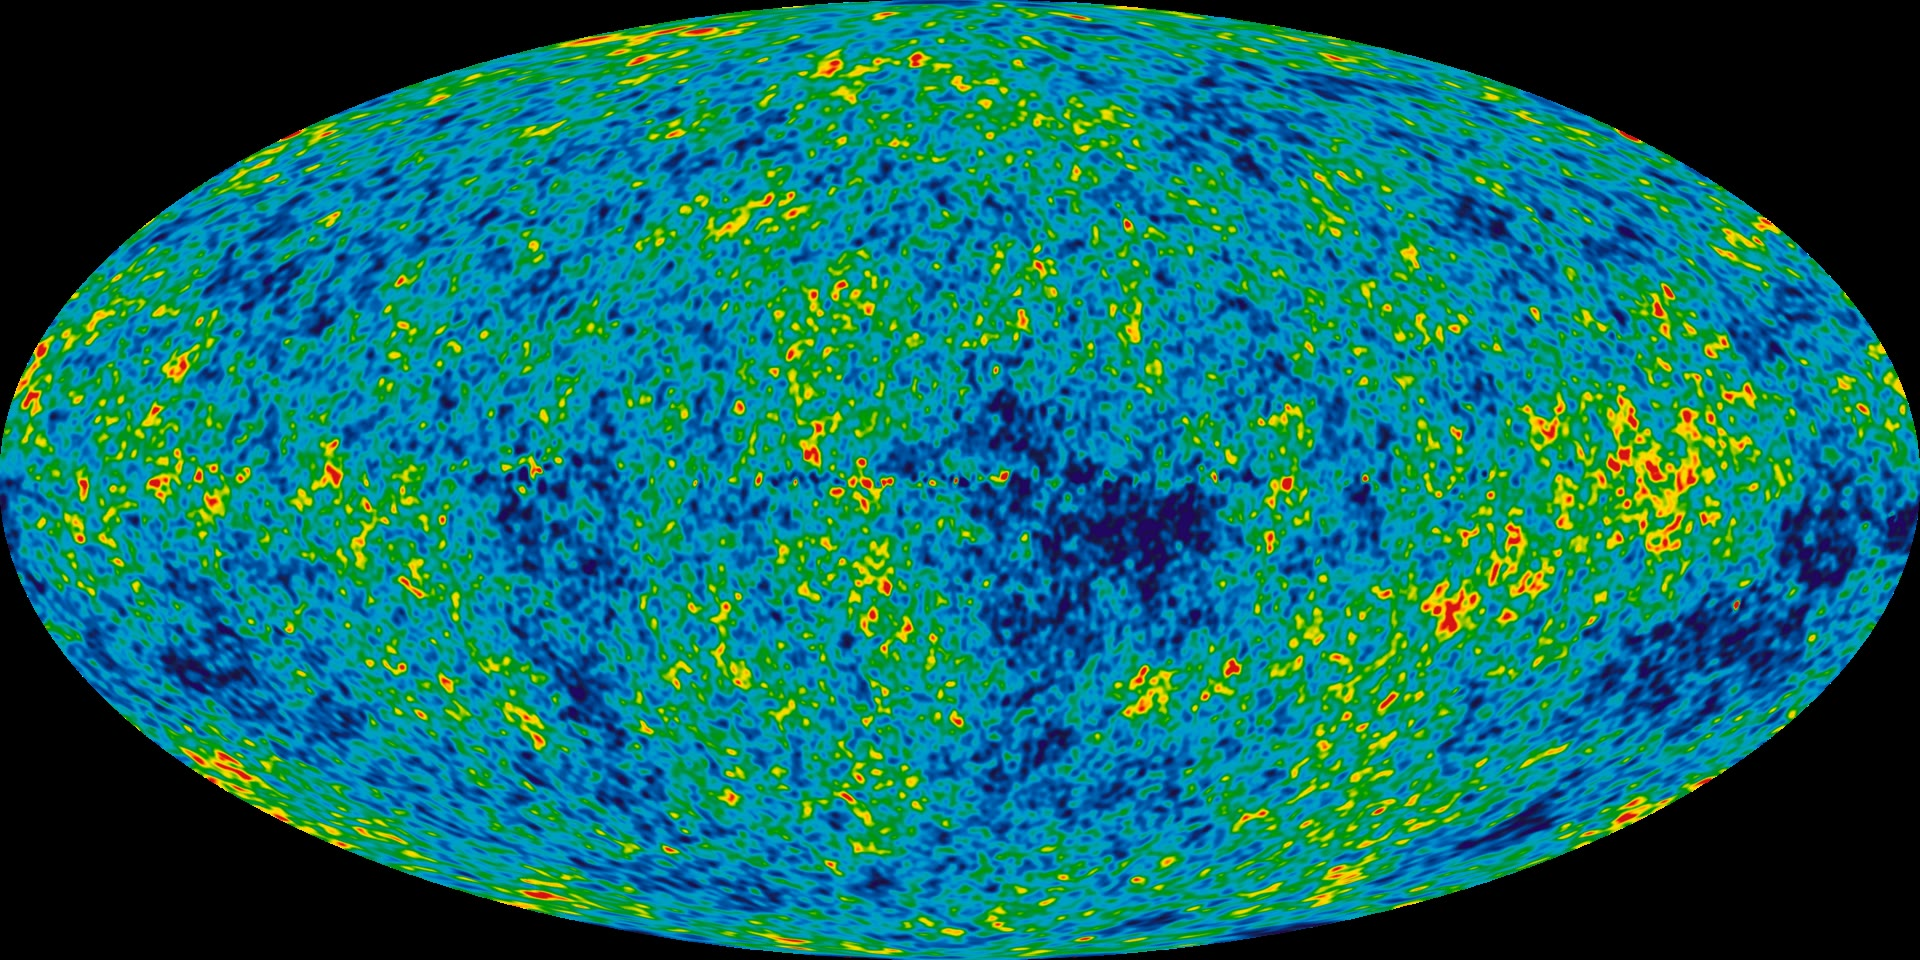
\includegraphics[width=0.62\linewidth]{images/book5/photo-cmb-wmap.jpg}

{\small السماء كلها في الميكرويّات (NASA/WMAP، ملكية عامة): أي إشعاع بلانك للخلفية الكونية عند \qty{2.7}{K}، مرسومًا. والتنقيط جزء من $10^5$ --- أي بذور المجرّات، مطبوعةً على جسم هذا الفصل الأسود.}
\end{omfigure}

\section{مسألة: أقدم ضوء}

\begin{problem}[{مسألة نهاية الأسبوع --- قراءة خلفية الكون
الميكروية}]\label{pb:b3:photons-phonons:1}
صوّب أيّ مستقبِل موجات ميليمترية إلى أيّ رقعة من السماء يذكرْ
الإشارة نفسها: أي طيف بلانك عند $T =
\qty{2.72548(57)}{K}$، أملسَ من أيّ فرن بناه البشر.
وهو ومضة إعادة الالتحام في الكون
(\cref{exo:b3:grand-canonical:12})، ممطوطةً ألفًا ومئة ضعف،
ويحمل تعداد الكون. والمعطيات: $T_0 =
\qty{2.725}{K}$؛ و $n_\gamma = \num{2.03e7}\,T^3\,\unit{m^{-3}}$؛ و
$u = aT^4$ مع $a = \qty{7.56e-16}{J.m^{-3}.K^{-4}}$؛ وكثافة الباريونات
اليوم $n_{\text{b}} \approx \qty{0.25}{m^{-3}}$؛ والكثافة الحرجة
$\rho_{\text{c}} \approx \qty{8.6e-27}{kg/m^3}$.

\medskip\noindent\textbf{الجزء الأول --- الطيف.}
\begin{enumerate}
  \item احسب الطول الموجي الذروي للخلفية (بفين) وكثافة
        فوتوناتها في السنتيمتر المكعب.
  \item احسب كثافة طاقتها، بوحدة $\unit{J/m^3}$ وبوحدة
        $\unit{eV/cm^3}$، ونسبة مكافئها الكتلي من
        الكثافة الحرجة.
  \item طابق طيف COBE (1990) بلانكَ في حدود أجزاء قليلة من
        $10^4$ --- فصفّق الحضور للرسم. فلماذا يصعب هكذا شرح
        طيف \emph{حراري تامّ} من سماء خالية بأيّ شيء
        سوى ماضٍ ساخن كثيف؟
  \item وعند الإصدار كوّنت الفوتونات نفسها جسمًا أسود عند \qty{3000}{K}:
        تحقق من عامل المطّ $1 + z =
        T_{\text{عندئذٍ}}/T_0$.
  \item ولماذا صار الكون شفافًا عند تلك الدرجة بالضبط
        (تذكّر أيّ توازن في
        \cref{ch:b3:grand-canonical} انطفأ)؟
  \item سماء الليل مظلمة (وهي مفارقة أولبرز في الفلك
        القديم): فبأيّ معنًى دقيق تكون في الواقع
        \emph{ساطعة} --- وعند أيّ طول موجي ودرجة حرارة؟
\end{enumerate}

\medskip\noindent\textbf{الجزء الثاني --- التعداد.}
\begin{enumerate}[resume]
  \item احسب نسبة الفوتونات إلى الباريونات $\eta^{-1} =
        n_\gamma/n_{\text{b}}$.
  \item وذلك العدد --- نحو ملياري فوتون لكل بروتون ---
        من معطيات علم الكون الأساسية: اذكر ما الذي يقيسه
        عن لاتناظر المادة--اللامادة (وتذكّر
        \cref{exo:b3:grand-canonical:12}: فالفوتونات أكثرها
        نواتج فناء).
  \item قارن كثافة طاقة الخلفية بكثافة ضوء النجوم
        ($\sim\qty{2e-15}{J/m^3}$ متوسَّطةً على الكون):
        فأيّ ضوء يهيمن على الكون؟
  \item والخلفية تفوق، بالفوتونات، كلَّ ما أشرقت به النجوم
        قط: فلماذا يجعل هذا الكونَ الفتيّ
        ``مهيمَنًا بالإشعاع''، وما الذي تولّى بعدئذٍ (بمقارنة
        تحجيمَي $T^4$ و $T^3$ بمقدار $a^{-3}$ للمادة)؟
  \item قدّر عهد تساوي المادة والإشعاع: فمع كثافة
        الإشعاع محجَّمةً وفق $(1+z)^4$ والمادة وفق
        $(1+z)^3$، ومع نسبة اليوم
        $u_{\text{rad}}/\rho_{\text{m}}c^2 \approx 1/3400$، جد
        $z_{\text{تعادل}}$.
  \item وقد انفصلت النيوترينوات أبكر وبردت أكثر قليلًا
        (إذ فاتها إعادة تسخين فناء $e^+e^-$ في
        \cref{exo:b3:grand-canonical:12}): فالمتنبَّأ به
        $T_\nu = (4/11)^{1/3}T_\gamma$ --- احسبه، و
        تعجّبْ من تنبؤ ببحر نيوترينوات عند \qty{1.95}{K}
        لم يكشفه أحد مباشرةً بعد.
\end{enumerate}

\medskip\noindent\textbf{الجزء الثالث --- اللاتماثلات المناحية.}
\begin{enumerate}[resume]
  \item الخفية أسخن بمقدار \qty{3.4}{mK} في اتجاه و
        أبرد في المقابل: فسّر ذلك بفيزياء دوبلر في
        \cref{ch:b3:relativistic-kinematics} واستخرج
        سرعتنا ($\Delta T/T = v/c$).
  \item وبعد إزالة ذلك القطب الثنائي، تبقى تموّجات $\Delta T/T \sim
        \num{e-5}$ (COBE سنة 1992، ثم WMAP، ثم بلانك): فماذا
        ترسم عند $z = 1100$؟
  \item وتلك البذور الكثافية $10^{-5}$ نمت مجرات: فلماذا
        تضخّم الثقالة الزيادات الكثافية (بأيّ عدم استقرار)،
        ولماذا احتاج النموّ إلى تساوي المادة والإشعاع كي يبدأ جدّيًّا؟
  \item وحجم أقوى تموّج (نحو درجة واحدة على السماء)
        طول موجي صوتي --- أي صوت في بلازما
        الفوتونات والباريونات (وهو غاز هذا الفصل مع
        أمواج \cref{ch:b3:continuum-elasticity}!): فما الذي يضع
        مقياسه (أي المسافة التي يقطعها الصوت قبل
        إعادة الالتحام)؟
  \item وقياس تلك الزاوية قياسًا إلى المقياس الفيزيائي المعلوم
        يثلّث هندسة الكون: اذكر
        النتيجة (مسطَّح، بدقة بالمئة).
  \item القطب الأحادي عند \qty{2.7}{K}، والقطب الثنائي عند \qty{3}{mK}، و
        تموّجات \num{e-5}: رتّب ما علّمه كلٌّ منها (ماضٍ ساخن؛
        وحركتنا؛ وبذور كل شيء وهندسته).
\end{enumerate}

\medskip\noindent\textbf{الجزء الرابع --- الإرث.}
\begin{enumerate}[resume]
  \item وجد بنزياس وويلسون الإشارة سنة 1965 ضجيجَ هوائي
        لا يُزال (بعد طرد الحمام): فلماذا
        كان فائض \emph{متماثل المناحي} مستقلّ الفصول عند
        \qty{3}{K} غير قابل للشرح بأيّ مصدر محلي أو مجرّي؟
  \item ونحو $1\%$ من تشويش تلفاز تناظري غير مضبوط
        كان هذه الإشارة: تأمّل في جملة واحدة.
  \item وتمرّ الخلفية عبر عناقيد المجرّات فتُركل قليلًا
        إلى تواتر أعلى بالإلكترونات الساخنة (وهو أثر
        سونييف--زلدوفيتش): فلماذا يجعل هذا العناقيد
        مرئيةً \emph{ظلالًا} عند التواتر المنخفض، وما ميزة
        ذلك الظلّ الخاصة (استقلاله عن
        البعد)؟
  \item وتصطاد جبهة اليوم استقطاب الخلفية بحثًا عن
        بصمة الأمواج الثقالية البدئية: فأيّ فصول
        من هذا الكتاب يزوّجها ذلك الاكتشاف
        (استقطاب \cref{ch:b3:covariant-electromagnetism}، و
        أمواج الثقالة)؟
  \item احسب تدفق فوتونات الخلفية عبر جسمك
        ($n_\gamma c/4$ لكل وحدة مساحة، \omterm{def:b3:scattering-theory:cross-section}{ومقطع} الجسم
        $\sim\qty{0.5}{m^2}$): فكم أثرًا من آثار الانفجار العظيم
        يعبرك في الثانية؟
  \item والخلفية تخصّ مرجعًا ساكنًا واحدًا (وهو الذي يتلاشى فيه
        القطب الثنائي): اشرح لماذا \emph{لا} يناقض هذا
        النسبية --- فأيّ صنف من المراجع تفضّله
        محتويات المادة لا القوانين؟
  \item لخّص النتيجة الموسومة: منحني بلانك عند $2.725$ كلفن
        يملأ السماء --- $411$ فوتونًا في السنتيمتر
        المكعب، ومليارين لكل باريون، وذروة عند
        \qty{160}{GHz} --- وهو الوصل الحراري للبداية
        الساخنة: أي الفيزياء الإحصائية حجرَ أساس
        علم الكون.
\end{enumerate}
\end{problem}
